

\section{Schliessende Statistik - Parameter- / Intervallschätzung}

\subsection{Zufallsstichproben}

\begin{concept}{Grundlagen der Zufallsstichproben}\\
Die Grundgesamtheit ist eine Menge von gleichartigen Objekten oder Elementen. Sie kann endlich oder unendlich viele Objekte enthalten.

Eine Stichprobe vom Umfang $n$ wird entnommen, um Informationen über die Grundgesamtheit zu gewinnen. Dies ist oft notwendig, da der Zeit- und Kostenaufwand für eine Vollerhebung zu hoch ist
\end{concept}

\begin{definition}{Einfache Zufallsstichprobe}\\
Eine einfache Zufallsstichprobe vom Umfang $n$ ist eine Folge von Zufallsvariablen $X_1, X_2, \ldots, X_n$ (Stichprobenvariablen). Dabei bezeichnet $X_i$ die Merkmalsausprägung des $i$-ten Elements in der Stichprobe.

Die beobachteten Merkmalswerte $x_1, x_2, \ldots, x_n$ der $n$ Elemente sind Realisierungen der Zufallsvariablen und heißen Stichprobenwerte.

Wichtige Eigenschaften:
\begin{itemize}
  \item Alle Stichprobenvariablen sind stochastisch unabhängig
  \item Alle $X_i$ folgen derselben Verteilung $F(x)$ der Grundgesamtheit
\end{itemize}
\end{definition}

\subsection{Parameterschätzungen}

\subsubsection{Schätzfunktionen}

\begin{definition}{Schätzfunktion}\\
Eine Schätzfunktion $\Theta = g(X_1,X_2,\ldots,X_n)$ ist eine spezielle Stichprobenfunktion zur Schätzung eines Parameters $\theta$ der Grundgesamtheit.

Der Schätzwert $\hat{\theta} = g(x_1,x_2,\ldots,x_n)$ ergibt sich durch Einsetzen der konkreten Stichprobenwerte.

$\theta$ ist der wahre, unbekannte Parameterwert der Grundgesamtheit.
\end{definition}

\begin{concept}{Grundlagen der Schätztheorie}\\
Die Schätztheorie befasst sich mit zwei Hauptproblemen:
\begin{itemize}
  \item Punktschätzung: Bestimmung eines einzelnen Schätzwerts
  \item Intervallschätzung: Bestimmung eines Vertrauensbereichs
\end{itemize}

Wichtige Begriffe:
\begin{itemize}
  \item $\theta$: Unbekannter Parameter der Grundgesamtheit
  \item $\Theta$: Schätzfunktion (Zufallsvariable)
  \item $\hat{\theta}$: Schätzwert (konkreter Wert)
  \item $n$: Stichprobenumfang
\end{itemize}
\end{concept}

\subsubsection{Kriterien für eine optimale Schätzfunktion}

\begin{concept}{Optimale Schätzfunktionen}\\
Eine Schätzfunktion sollte folgende Eigenschaften haben:

\begin{itemize}
    \item Erwartungstreu: $E(\Theta) = \theta$
    \item Effizient: Kleinste Varianz unter allen Schätzern $V(\Theta_1)<V(\Theta_2)$
    \item Konsistent: $E(\Theta) \to \theta$ und $V(\Theta) \to 0$ für $n \to \infty$\\
    $\rightarrow$ Grenzwert für $n \to \infty$ betrachten
\end{itemize}

\textbf{Interpretation:}
\begin{itemize}
  \item Erwartungstreue: im Mittel wird der richtige Wert geschätzt
  \item Effizienz: möglichst geringe Streuung der Schätzung
  \item Konsistenz: Schätzung wird mit wachsender Stichprobe genauer
\end{itemize}
\end{concept}

\begin{example2}{Beispiel Erwartungstreue einer Schätzfunktion}\\
Grundgesamtheit mit Erwartungswert $\mu$, Varianz $\sigma^2$ und Zufallsstichprobe $X_1, X_2, X_3$. \\Die folgende Schätzfunktion ist gegeben:
$
\Theta_1=\frac{1}{3} \cdot(2X_1+X_2)
$\\
Ist diese Schätzfunktion erwartungstreu (wahrer Parameter: $\mu$)?
$$
\begin{gathered}
E(\Theta_1)=E(\frac{1}{3} \cdot(2X_1+X_2))=\frac{1}{3} \cdot(2E(X_1)+E(X_2)) \\
E(\Theta_1)=\frac{1}{3} \cdot(2\mu+\mu)=\frac{3\mu}{3}=\mu
\end{gathered}
$$
\textit{Da $E(\Theta_1)=\mu$ ist die Funktion erwartungstreu.}
\end{example2}

\begin{example2}{Effizienz einer Schätzfunktion}\\
Grundgesamtheit mit Erwartungswert $\mu$, Varianz $\sigma^2$ und Zufallsstichprobe $X_1, X_2, X_3$. Gegeben ist die Schätzfunktion:
$\Theta_1=\frac{1}{3} \cdot(2X_1+X_2)$
\vspace{1mm}\\
\textbf{Berechnung der Effizienz:}
\vspace{1mm}\\
$V(\Theta_1)=V(\frac{1}{3} \cdot(2X_1+X_2))=\frac{1}{9} \cdot V(2X_1+X_2)$\\
$= \frac{1}{9} \cdot (V(2X_1)+V(X_2))=\frac{1}{9} \cdot (4V(X_1)+V(X_2))$\\
$= \frac{1}{9} \cdot (4\sigma^2+\sigma^2)=\frac{5\sigma^2}{9}$
\vspace{1mm}\\
Die Effizienz der Schätzfunktion ist also $\frac{5\sigma^2}{9}$.
\end{example2}

\subsubsection{Wichtige Schätzfunktionen}
%TODO: nicer formatting
\begin{theorem}{Schätzfunktionen für wichtige Parameter}\\
\textbf{Erwartungswert:}
\vspace{-4mm}\\
\[\bar{X} = \frac{1}{n}\sum_{i=1}^n X_i \qquad \hat{\mu} = \bar{x} = \frac{1}{n}\sum_{i=1}^n x_i\]
\vspace{-4mm}\\
Eigenschaften:
\begin{itemize}
  \item Erwartungstreu: $E(\bar{X}) = \mu$
  \item Konsistent: $V(\bar{X}) = \frac{\sigma^2}{n} \to 0$ für $n \to \infty$
\end{itemize}
\vspace{1mm}
\textbf{Varianz:}
\vspace{-4mm}\\
\[S^2 = \frac{1}{n-1}\sum_{i=1}^n (X_i-\bar{X})^2 \qquad \hat{\sigma}^2 = s^2 = \frac{1}{n-1}\sum_{i=1}^n (x_i-\bar{x})^2\]
\vspace{-2mm}\\
Eigenschaften:
\begin{itemize}
  \item Erwartungstreu: $E(S^2) = \sigma^2$
  \item Konsistent: $V(S^2) \to 0$ für $n \to \infty$
\end{itemize}
\vspace{1mm}
\textbf{Anteilswert:} (bei Bernoulli-Verteilung)
\vspace{-2mm}\\
\[\bar{X} = \frac{1}{n}\sum_{i=1}^n X_i \qquad \hat{p} = \bar{x} = \frac{1}{n}\sum_{i=1}^n x_i\]
\end{theorem}

\subsection{Vertrauensintervalle}

\begin{definition}{Vertrauensintervall}\\
Ein Vertrauensintervall $[\Theta_u,\Theta_o]$ zum Niveau $\gamma$ ist ein zufälliges Intervall mit:

\[P(\Theta_u \leq \theta \leq \Theta_o) = \gamma\]

$\gamma$: Vertrauensniveau (statistische Sicherheit)\\
$\alpha = 1-\gamma$: Irrtumswahrscheinlichkeit\\
$\Theta_u, \Theta_o$: Unter- und Obergrenze
\end{definition}




\begin{KR}{Konstruktion eines Vertrauensintervalls}\\
1. Verteilungstyp bestimmen:
   \begin{itemize}
     \item Parameter ($\mu$ oder $\sigma^2$)
     \item $\sigma^2$ bekannt oder unbekannt
   \end{itemize}

2. Quantile bestimmen:
   \begin{itemize}
     \item $\gamma$ und $\alpha$ beachten
     \item Richtige Tabelle wählen
     \item Freiheitsgrade $f=n-1$ beachten
   \end{itemize}

3. Intervallgrenzen berechnen:
   \begin{itemize}
     \item Standardfehler berechnen
     \item Grenzen $\Theta_u$ und $\Theta_o$ bestimmen
   \end{itemize}
\end{KR}



\begin{example2}{Beispiel: Konstruktion eines Vertrauensintervalls (Normalverteilung)}\\
Gegeben: \textbf{normalverteilte} Zufallsvariable $X$ mit unbekanntem Parameter $\mu$ und bekannter Varianz $\sigma^2$. $\gamma = 0.95$. 

\textbf{Aufgabe:} Konstruiere ein Vertrauensintervall für den Mittelwert $\mu$.

\textbf{1. Verteilungstyp bestimmen}
siehe \textcolor{purple}{\textbf{Übersicht Vertrauensintervalle}}
\vspace{2mm}\\
\textbf{2. Gleichung aufstellen}
Die Schätzfunktion für $\mu$ liefert Ausgangspunkt für Vertrauensintervall, ausgehend von diesem Punkt berechnen wir die Grenzen.
\vspace{1mm}\\
Die Grenzen sollen symmetrisch um $\bar{X}$ liegen. Wir suchen also eine Schranke $e$ so dass gilt:
$$
P(\bar{X}-e \leq \mu \leq \bar{X}+e)=\gamma \text{ bzw. } P(|\bar{X}-\mu| \leq e)=\gamma(*)
$$

\textbf{3. Standardisierung}
Nach dem Zentralen Grenzwertsatz ist $\bar{X}$ normalverteilt mit $E(\bar{X})=\mu$ und $\operatorname{Var}(\bar{X})=\frac{\sigma^2}{n}$. Damit wir Wahrscheinlichkeiten bestimmen können, müssen wir statt $\bar{X}$ die standardisierte Zufallsvariable $U=\frac{\hat{X}-\mu}{\sigma / \sqrt{n}}$ verwenden; $U$ ist standardnormalverteilt.
Die Gleichung (*) lässt sich umformen zu:
$
P(|U| \leq \frac{e}{\sigma / \sqrt{n}})=\gamma
$

\textbf{4. $c$ bestimmen}

\begin{minipage}{0.5\linewidth}
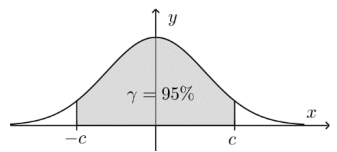
\includegraphics[width=\linewidth]{images/bsp_vertrauensintervall.png}
\end{minipage}
\begin{minipage}{0.5\linewidth}
Die Illustration zeigt die Situation, dabei ist $c=\frac{e}{\sigma / \sqrt{n}}$.
\vspace{1mm}\\
Wir suchen also: \\das $c$ mit $\phi(c)=\frac{1+\gamma}{2}=0.975$.
\end{minipage}

Aus der Standardnormalverteilungstabelle erhalten wir $c=1.96$.
\vspace{2mm}\\
\textbf{5. Intervallgrenzen berechnen} $e=c \cdot \frac{\sigma}{\sqrt{n}}$
\vspace{2mm}\\
\textbf{Formeln für die Stichprobenfunktionen und Grenzen:}
$$
\Theta_u=\bar{X}-\underbrace{c \cdot \frac{\sigma}{\sqrt{n}}}{e}, \quad \Theta_o=\bar{X}+\underbrace{c \cdot \frac{\sigma}{\sqrt{n}}}{e}
$$
\end{example2}



\begin{KR}{Bestimmung des Stichprobenumfangs}\\
1. Gegebene Verteilung und Parameter:
   \begin{itemize}
     \item Normalverteilung mit $\sigma^2$ bekannt
     \item Vertrauensniveau $\gamma$
     \item Maximal zulässige Intervallbreite $d$
   \end{itemize}

2. Kritischen Wert bestimmen:
   \begin{itemize}
     \item $p = \frac{1+\gamma}{2}$
     \item $c = u_p$ für Normalverteilung
   \end{itemize}

3. Stichprobenumfang berechnen:
   \begin{itemize}
     \item $n \geq (\frac{2c\sigma}{d})^2$
     \item Auf nächste ganze Zahl aufrunden
   \end{itemize}

4. Bei unbekannter Varianz:
   \begin{itemize}
     \item Vorerhebung durchführen
     \item Varianz schätzen
     \item t-Verteilung statt Normalverteilung
   \end{itemize}
\end{KR}

\begin{example2}{Beispiel: Stichprobenumfang bestimmen}\\
Ein Prozess produziert Teile mit bekannter Standardabweichung $\sigma = 0.5$ mm. Der Mittelwert soll mit einer Genauigkeit von $\pm 0.2$ mm bei einem Vertrauensniveau von 99\% geschätzt werden.

1. Gesucht:
   \begin{itemize}
     \item Intervallbreite $d = 0.4$ mm
     \item $\gamma = 0.99$
   \end{itemize}

2. Kritischer Wert:
   \begin{itemize}
     \item $p = \frac{1+0.99}{2} = 0.995$
     \item $c = u_{0.995} = 2.576$
   \end{itemize}

3. Stichprobenumfang:
   \begin{itemize}
     \item $n \geq (\frac{2 \cdot 2.576 \cdot 0.5}{0.4})^2 = 41.47$
     \item $n = 42$ (aufgerundet)
   \end{itemize}
\end{example2}

\begin{remark}
\begin{minipage}[t]{0.5\textwidth}
\begin{itemize}
  \item $c$: Quantil der Verteilung
  \item $p$: Wahrscheinlichkeit für Quantil
  \item $f$: Freiheitsgrade
  \item $s$: Schätzwert für $\sigma$
  \item $S^2$: Schätzvarianz
  \item $n$: Stichprobenumfang
  \item $\bar{X}$: Stichprobenmittelwert
  \item $\gamma$: Vertrauensniveau
  \item $\alpha$: Irrtumswahrscheinlichkeit
\end{itemize}
\end{minipage}
\begin{minipage}[t]{0.5\textwidth}
\begin{itemize}
  \item $\mu$: Wahre Parameter der \\Grundgesamtheit
  \item $\sigma$: Wahre Varianz der \\Grundgesamtheit
  \item $\Theta_u, \Theta_o$: Unter- und Obergrenze \\des Intervalls
  \item $c_1, c_2$: Quantile der Verteilung
  \item $p_1, p_2$: Wahrscheinlichkeiten \\für Quantile
\end{itemize}
\end{minipage}
\end{remark}

\begin{remark}
$\gamma$ gibt Wahrscheinlichkeit an, dass das Intervall den wahren Parameter $\theta$ enthält. Irrtumswahrscheinlichkeit $\alpha=1-\gamma$.

\textbf{Beispiel:} $\gamma=0.95$ bedeutet, dass in 95\% der Fälle das Intervall den wahren Parameter enthält $\rightarrow \alpha=0.05$

Meist kann das Vertrauensniveau $\gamma$ frei gewählt werden ($\alpha$ möglichst klein). Häufig wird $\gamma=0.95$ oder $\gamma=0.99$ gewählt.
\end{remark}

\begin{example2}{Beispiel: Berechnung eines Vertrauensintervalls (t-Verteilung)}\\
Geben Sie das Vertrauensintervall für $\mu$ an ($\sigma^2$ unbekannt). Gegeben sind:
$$
n=10, \quad \bar{x}=102, \quad s^2=16, \quad \gamma=0.99
$$

\begin{enumerate}
  \item Verteilungstyp mit Param $\mu$ und $\sigma^2$ unbekannt $\rightarrow$ T-Verteilung
  \item $f=n-1=9$, $p=\frac{1+\gamma}{2}=0.995$, $c=t_{(p;f)}=t_{(0.995;9)}=3.25$
  \item $e=c \cdot \frac{S}{\sqrt{n}}=4.111$, $\Theta_u=\bar{X}-e=97.89$, $\Theta_o=\bar{X}+e=106.11$
\end{enumerate}
\end{example2}

\begin{formula}{Übersicht Vertrauensintervalle} zum Niveau $\gamma$
\vspace{2mm}\\
  \renewcommand{\arraystretch}{1.7}
\begin{adjustbox}{angle=90}
\begin{tabular}{|l|l|l|l|l|l|l|}
\hline
& Verteilung der & Param. & Schätzfunktionen & standardisierte  & Verteilung und   & Intervallgrenzen \\
& Grundgesamtheit &  &  &  Zufallsvariable &  benötigte Quantile &  \\
\hline
\multirow{2}{1mm}{1} & Normalverteilung  & \multirow{2}{5mm}{$\mu$} & \multirow{2}{25mm}{$\bar{X}=\frac{1}{n}\cdot \sum_{i=1}^{n} X_i$} & \multirow{2}{25mm}{$U = \frac{\bar{X}-\mu}{\sigma/\sqrt{n}}$} & Standardnormalverteilung (Tab.2) & \multirow{2}{20mm}{$\bar{x} \pm c\frac{\sigma}{\sqrt{n}}$} \\
 &  ($\sigma^2$ bekannt) &  &  &  & $c=u_p$ mit $p=\frac{1+\gamma}{2}$ &  \\
\hline
\multirow{2}{1mm}{2} & Normalverteilung & \multirow{2}{5mm}{$\mu$} & $\bar{X}=\frac{1}{n}\cdot \sum_{i=1}^{n} X_i$ & \multirow{2}{25mm}{$T = \frac{\bar{X}-\mu}{S/\sqrt{n}}$} & t-Verteilung (Tab.4) $f=n-1$ & \multirow{2}{20mm}{$\bar{x} \pm c\frac{s}{\sqrt{n}}$} \\
 &  ($\sigma^2$ unbek.) &  & \multirow{2}{35mm}{$S^2 = \frac{1}{n-1}\cdot \sum_{i=1}^{n} (X_i - \bar{X})^2$} &  & $c=t_{p,f}$ mit $p=\frac{1+\gamma}{2}$ &  \\
 & & & & & & \\
\hline
\multirow{2}{1mm}{3} & Normalverteilung & \multirow{2}{5mm}{$\sigma^2$} & $\bar{X}=\frac{1}{n}\cdot \sum_{i=1}^{n} X_i$ & \multirow{2}{25mm}{$Z = (n-1)\frac{S^2}{\sigma^2}$} & $\chi^2$-Verteilung (Tab.3) $f=n-1$ & \multirow{2}{20mm}{$\Theta_u = \frac{(n-1)s^2}{c_2}$} \\
 &  &  & \multirow{2}{35mm}{$S^2 = \frac{1}{n-1}\cdot \sum_{i=1}^{n} (X_i - \bar{X})^2$} &  & $c_1=z_{p_1,f}$, $p_1 = \frac{1+\gamma}{2}$ &  \\
 & & & & & $c_2=z_{p_2,f}$, $p_2 = \frac{1-\gamma}{2}$ & $\Theta_o =\frac{(n-1)s^2}{c_1}$\\
\hline
\multirow{2}{1mm}{4} & Bernoulli-Verteilung & \multirow{2}{5mm}{$p$} & $\bar{X}=\frac{1}{n}\cdot \sum_{i=1}^{n} X_i$ & \multirow{2}{25mm}{$U = \frac{\bar{X}-p}{\sqrt{\frac{p(1-p)}{n}}}$} & Standardnormalverteilung (Tab.2) & \multirow{2}{20mm}{$\bar{x} \pm c\sqrt{\frac{\bar{x}(1-\bar{x})}{n}}$} \\
 & Anteilsschätzung &  & $X_i$ $0/1$-wertig  &  & $c=u_p$ mit $q=\frac{1+\gamma}{2}$ &  \\
 & & & $P(X_i=1)=p$ & & & \\
\hline
5 & beliebig mit n $\geq$ 30 & $\mu$, $\sigma^2$ & \multicolumn{4}{|c|}{Wie im Fall 1 (gegebenenfalls mit $s$ als Schätzwert), bzw. im Fall 3} \\
\hline
\end{tabular}
\end{adjustbox}
\end{formula}